%% !TEX root = manual.tex

\section{Network Model}
\label{sec:tutorial:networkmodel}

\subsection{Packet}
\label{subsec:tutorial:packet}
The packet model is the simplest and most intuitive of the congestion models for simulating network traffic.
The physics correspond naturally to a real machine: messages are broken into small chunks (packets) and routed individually through the network.
When two messages compete for the same channel (Figure \ref{fig:tutorial:congestion}A), arbitration occurs at regular intervals to select which packet has access.
Packets that lose arbitration are delayed, leading to network congestion.
In \sstmacro, the packet model is still \emph{coarse-grained}.
In a real machine, packet sizes can be very small (100 B).
Additionally, arbitration can happen on flits (flow control units), an even smaller unit than the packet.
Flit-level arbitration or even 100B packet arbitration is far too fine-grained to do system-level simulation. 
While packet size is tunable in \sstmacro, the simulator is designed for coarse-grained packet sizes of 1 KB to 8 KB.
The same flow control (routing, arbitration, congestion avoidance) is performed on coarse-grained packets, but some accuracy is lost.

The coarse-grained packet model has two main sources of error.  
First, coarse-grained packets systematically overestimate (de)serialization latency.
Before a packet can be forwarded to its next destination, it must be completely deserialized off the network link into a buffer.
In a real machine, data can be forwarded on a flit-by-flit basis, efficiently pipelining packets.
Flits that would send in a real system are artificially delayed until the rest of the coarse-grained packet arrives.
Second, coarse-grained packets exclusively reserve network links for the entire length of the packet.
In a real machine, two packets could multiplex across a link on a flit-by-flit basis.

\begin{figure}[h]
\centering
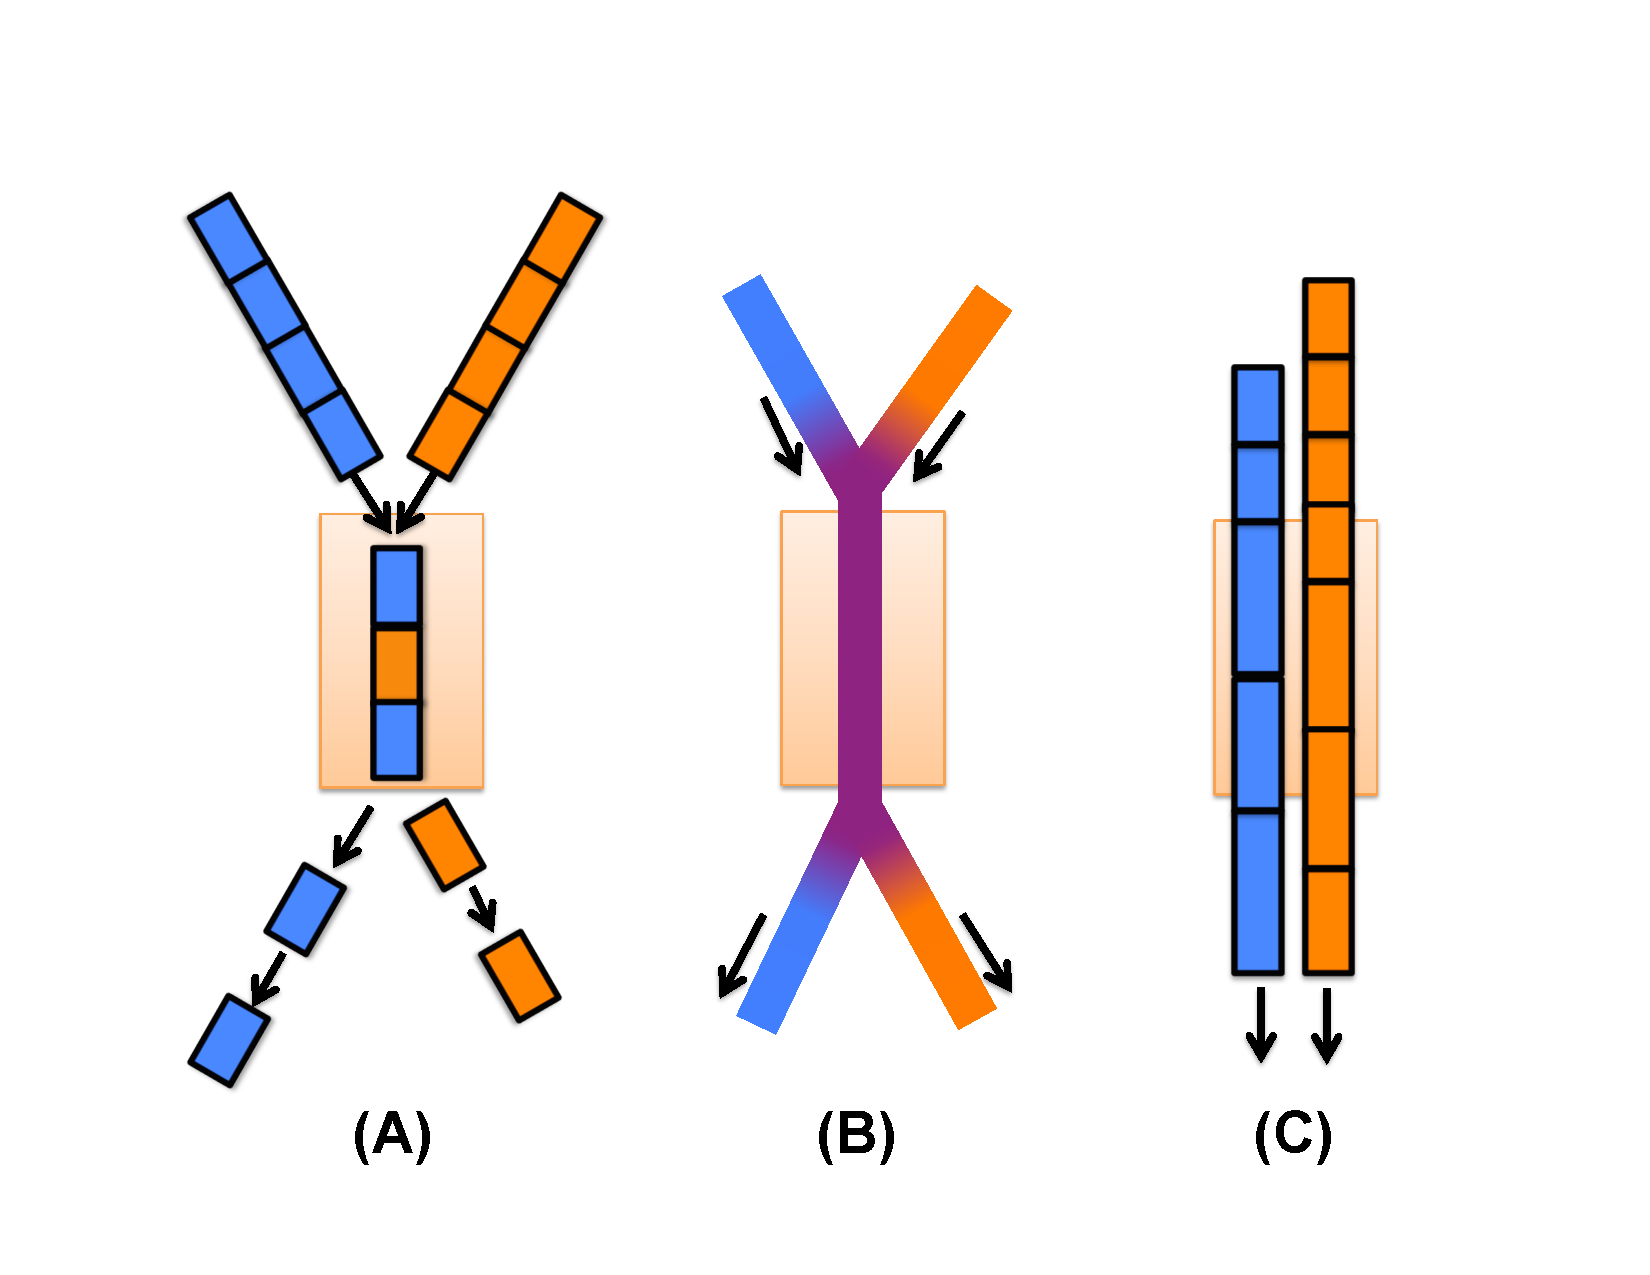
\includegraphics[width=0.5\textwidth]{figures/network/congestion.pdf}
\caption{Schematic of two messages competing for same channel in the different \sstmacro congestion models. (A) Packet Model  (B) Flow Model (C) Packet-flow Model }
\label{fig:tutorial:congestion}
\end{figure}

\subsection{Flow}
\label{subsec:tutorial:flow}
The flow model, in simple cases, corrects the most severe problems of the packet model.
Instead of discrete chunks, messages are modeled as fluid flows moving through the network (Figure \ref{fig:tutorial:congestion}B).
Congestion is treated as a fluid dynamics problem, sharing bandwidth between competing flows.
Without congestion, a flow only requires a FLOW START and FLOW STOP event to be modeled (see tutorial on discrete event simulation in \ref{sec:tutorial:des}).
While the packet model would require many, many events to simulate a 1 MB message, the flow model might only require two.
With congestion, flow update events must be scheduled whenever congestion changes on a network link.  
For limited congestion, only a few update events must occur.
The flow model also corrects the latency and multiplexing problems in the packet model, providing higher-accuracy for coarse-grained simulation.

The flow model starts to break down for large systems or under heavy congestion.
In the packet model, all congestion events are ``local'' to a given router.  
The number of events is also constant in packet models regardless of congestion since we are modeling a fixed number of discrete units.
In flow models, flow update events can be ``non-local,'' propagating across the system and causing flow update events on other routers.
When congestion occurs, this ``ripple effect'' can cause the number of events to explode, overwhelming the simulator.
For large systems or heavy congestion, the flow model is actually much slower than the packet model. Support for this model has been completely removed.

%\sstmacro actually implements a modified ``fast-flower'' model that introduces new approximations to avoid the ripple effect.
%With modest congestion, the approximations are still relatively accurate and should produce good results.
%For more details on flow parameters, see the \inlineshell{hopper_flow.ini} file in the \inlineshell{configurations} folder in the \sstmacro source.
%The flow model can also be explored via the GUI (see \ref{sec:basicgui}).

\subsection{Packet-flow}
\label{subsec:tutorial:train}
Packet-flow is a hybrid-model of flow and packet, trying to correct the latency errors in the packet model while avoiding the ripple effect of the flow model.
Much like packets, the packet-flow model begins by converting messages into many discrete chunks of fixed size.
In contrast to the packet model, channel arbitration is not exclusive.  
When multiple packets compete for a channel, each packet ``samples'' the current congestion (Figure \ref{fig:tutorial:congestion}C).
Based on congestion, the packets estimates its bandwidth and latency.
If low congestion is sampled, high-bandwidth is assigned (short packet in the figure).
If high congestion is sampled, low-bandwidth is assigned (long packet in the figure).

The packet-flow model corrects the two most important packet model errors.
Once bandwidth has been assigned, the packet can immediately be forwarded to the next router, producing accurate latencies.
The sampling procedure also allows two packets to multiplex across a channel.
Because messages are broken into discrete chunks, the number of events per message is constant regardless of congestion, avoiding the ripple effect.

For more details on packet-flow parameters, see the \inlineshell{hopper_amm.ini} files in the \inlineshell{configurations} folder in the \sstmacro source.

